\chapter{Fundamentals}

\section{Introduction}

Welcome to competitive programming! If you know a bit about coding and you're curious about programming contests, then you're in the right place. We'll start these notes with some basic background: what happens during a programming contest, which skills they train, and how to practice and become better. In the second part of this section, we'll walk through an example contest problem together. As you move forward, these notes will both guide you through key algorithmic and data structural ideas and provide interesting problems for you to think about. We'll try to challenge you, make you a better thinker and programmer, and give you a sense for how the foundational concepts in computer science are intricately connected. And if you have questions or feedback about anything, feel free to hit us up at \mailto{@gmail.com}. We hope you'll enjoy the world of competitive programming as much as we have. Have fun with it!

\subsection{What is Competitive Programming?}

A programming contest typically consists of a collection of problems and a time limit within which they must be solved. To solve a problem, you'll have to code a program that reads some parameters as input and produces an output of the desired format. You'll then submit your code to a \emph{judging server}, which is a server that compiles your code and executes it on a set of \emph{test cases}. To pass, your program must solve each test case using only predetermined amounts of \emph{time} and \emph{memory}. That is, your program must be \textit{efficient}. Furthermore, your program must be \textit{correct}. To check correctness, the output for each test case is either compared to the output of a correct program written by the contest organizers or plugged into a verifier that checks that your output satisfies the desired conditions. So as a contestant, your job will be to find an efficient algorithm, write correct code, and submit.

This is just a very general description of programming contests. Each contest has its particularities in terms of scoring and the feedback you get on your submissions. Some contests will only mark your submission as correct if it correctly solves every test case, while others will give you partial credit for every test case you get correct.  Some contests will also execute your submissions in real time, so you'll know if your code is correct within seconds, while others will only judge your final submissions after the contest is over. But the commonalities of these contests are in the skills they select for and train.

Problem solving is possibly the most important skill you can learn. This skill, and not whether you can crank out code quickly, is what interesting programming contests are about. You'll be given problems you'll have no idea how to solve, and you'll want to creatively reason about these problems and discover efficient solutions. Of course, being able to write clean, accurate code is also of high importance, since it is your code, not the solution in your head, that gets judged. For programming language, we recommend (and our notes will cover) coding in \emph{Java} or \emph{C++}. Finally, a solid understanding of algorithms and data structures will give you the tools you'll need to crack these problems. This combination of problem solving, coding, and algorithmic thinking will get you a long way in programming contests, and you'll definitely be able to apply them elsewhere too.

We'll do our best to teach you these skills by providing you with notes that show you the important algorithmic and data structural ideas, giving you pointers on how to write code, and presenting you with problems that will solidify your knowledge. I cannot emphasize how important solving the problems and writing the code is for your growth. Try to avoid reading solutions until you've given the problem a genuine shot and feel like you've stopped making progress. And if you do read a solution, think about how you'll be able to solve a similar problem the next time it appears. After you solve a problem, code it up, and don't give up trying to fix and optimize your code until you get all test cases accepted. Think of each bug you find as another bug you'll never see again.

But there is only so much we can do. The challenging part---persevering with difficult problems, spending long hours spent debugging, and taking time from your busy day to code---is all on you.

\subsection{First Problem: Sliding Puzzles}

We'll now work through an example problem, adapted from a recent Codeforces contest. On the next page is a typical problem statement, with the problem description followed by input and output specifications and sample cases. Try to come up with a solution (and possibly write some code) before reading our analysis. As in the rest of these notes, we'll follow our analysis with some discussion of how to implement the solution and provide links to C++ and/or Java code.

\clearpage

\statement[Sliding Puzzles]{2s}{256MB}{%
  Bessie and her best friend Elsie each own a sliding puzzle. Each of their sliding puzzles consists of a $2\times 2$ grid and three tiles labeled $\mathcal A$, $\mathcal B$, and $\mathcal C$. The three tiles sit on top of the grid, with one grid cell left empty. To make a move, one slides a tile adjacent to the empty cell into the empty cell, as shown below:
  \begin{center}
    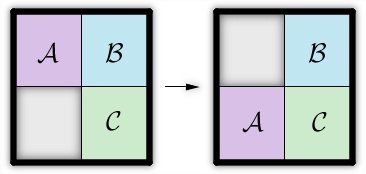
\includegraphics[scale=0.6]{images/sliding-puzzle.png}
  \end{center}
  Bessie and Elsie would like to know if there exists a sequence of moves that takes their puzzles to the same configuration. (Moves can be performed on both puzzles.) Two puzzles are considered to be in the same configuration if each tile is on top of the same grid cell in both puzzles. Since the tiles are labeled with letters, rotations and reflections are not allowed.
}{%
  The first two lines of the input consist of a $2\times 2$ grid describing the initial configuration of Bessie's puzzle. The next two lines contain a $2\times 2$ grid describing the initial configuration of Elsie's puzzle. The positions of the tiles are labeled $\mathtt A$, $\mathtt B$, and $\mathtt C$, while the empty cell is labeled $\mathtt X$. It is guaranteed that the input contains two valid descriptions of puzzles.
}{%
  Print \texttt{YES} if the puzzles can reach the same configuration. Otherwise, print \texttt{NO}.
}{\href{http://codeforces.com/contest/645/problem/A}{Codeforces 645A}}
\sample{%
  AB
  XC
  XB
  AC%
}{YES}
\sample{%
AB
XC
AC
BX%
}{NO}

\clearpage

We present two solutions to this problem. The first is the more ``obvious'' one, while the second shows how solutions can often be simplified through some thinking and some clever observations.

\begin{proof}[Solution 1]
  One straightforward approach to this problem is to notice that there are only $4! = 24$ possible  configurations that a puzzle could be in. Thus, for each puzzle in the input, it shouldn't be hard to find the list of configurations that the puzzle can reach. Once we have the lists of configurations, we can compare the two lists and check if they have an element in common. If they do, we output $\mathtt{YES}$; otherwise, we output $\mathtt{NO}$.

  To find the list of possible configurations, we maintain a list containing all of the possible configurations we have found so far. (This list starts off as the puzzle itself.) For every configuration in our list, we check if a single move can take us to a configuration we haven't seen before. Once we find a new configuration, we append it to the list and repeat. If there exist no such new configurations, then our list contains all possible configurations for that puzzle.
\end{proof}

However, this solution may be somewhat difficult to implement---we have to figure out how to nicely represent each configuration as a string and make moves to reach new configurations. Writing the code to find the list of possible configurations is also a bit complex. Instead, a simple observation can reduce the trickiness of the code significantly:

\begin{proof}[Solution 2]
  Notice that two puzzles can reach the same configuration if and only if the $\mathcal A$, $\mathcal B$, and $\mathcal C$ tiles appear in the same orientation---clockwise or counterclockwise---in the two puzzles. Thus, it suffices to check if the two puzzles have the same orientation. We can do so by writing down the tiles of each puzzle in clockwise order and checking if one string is a cyclic shift of the other.
\end{proof}

To implement the first solution, you might want to make your list of possible configurations a \emph{dynamic array}---that is, a Java \texttt{ArrayList} or a C++ \texttt{vector}. This will allow you to easily append elements to the list.

For the second solution, once we have the tiles in clockwise order, we'll want to check if one ordering is a cyclic shift of the other. Given two strings $s$ and $t$ of the same length, a clever way to do this is to check if $s$ is a substring of $t+t$. (Convince yourself that this is correct!) Take a look at a \href{http://codeforces.com/contest/645/submission/16801722}{C++} implementation of Solution 2 using this trick.

\section{More Problems!}
\label{sec:moreproblems}

Because problems are the most important thing in the world, below are a couple more for you to chew on. We'll cover solutions to these problems later in the chapter, but if you feel ready, try submitting your code on \href{http://codeforces.com}{Codeforces} first.

\statement[Vasily and Candles]{1s}{256MB}{%
  Vasily the programmer loves romance, so he plans to write code while bathed in the warm glow of candlelight. He has $a$ new candles, each of which burns for exactly one hour. Vasily is smart, so he can make a new candle from $b$ burnt out candles. Vasily wonders, for how many hours can his candles light up his room if he acts optimally?
}{%
  The input contains two integers, $a$ and $b$ ($1\le a\le 1000$ and $2\le b\le 1000$).
}{%
  Print a single integer---the maximum number of hours for which Vasily's candles can keep his room lit.
}{\href{http://codeforces.com/problemset/problem/379/A}{Codeforces 379A}}
\sample{4 2}{7}
\sample{6 3}{8}

\statement[Kefa and First Steps]{2s}{256MB}{%
  Kefa has started an Internet business $n$ days ago. On the $i$-th day $(1\le i\le n)$, he made a profit of $a_i$ dollars. Kefa loves progress, so he wants to know the length of the longest non-decreasing subsegment in her sequence of profits. (Here, a subsegment of a sequence denotes a contiguous subsequence $a_i,a_{i+1}\ldots,a_j$ ($i < j$).)
}{%
  The first line contains an integer $n$ ($1\le 10^5$). The second line contains $n$ integers $a_1,a_2,\ldots,a_n$ ($1\le a_i\le 10^9$).
}{%
  Print a single integer--the length of the maximum non-decreasing sequence in Kefa's profits.
}{\href{http://codeforces.com/problemset/problem/580/A}{Codeforces 580A}}
\sample{%
  6
  2 2 1 3 4 1%
}{3}
\sample{%
  3
  2 2 9%
}{3}

\section{Input and Output}

Now that you've familiarized yourself with what programming contest problems are like, let's get down to the details. The first part of solving any problem is reading the input correctly. As you may expect, doing so is very dependent on programming language. In this section, we'll cover input and output (I/O) in both Java and C++. Read our discussion for whichever one you plan to use.

\subsection{Java}
Here, we'll focus on Java I/O using \texttt{java.util.Scanner} and \texttt{java.io.PrintWriter}. There are two scenarios that you should be familiar with: standard I/O and file I/O. That is, interacting with \texttt{System.in/System.out} and files like \texttt{in.txt/out.txt}, respectively. You may have encountered standard I/O when you enter input and see output while running a program in the command line.

When using standard I/O, we can read from \texttt{System.in} using \texttt{java.util.Scanner} and output using \texttt{System.out.println}. To declare a new Scanner, simply call the constructor with \texttt{new Scanner(System.in)}. Here's a quick outline of Scanner methods:
\begin{center}
  \begin{tabularx}{0.75\textwidth}{|l|X|}
    \hline
    Method & Description \\ \hline
    \texttt{Scanner.next()} & Reads the next token in the input (i.e. up to a whitespace) and returns the token as a \texttt{string}. \\ \hline
    \texttt{Scanner.nextLine()} & Reads the input up to a line break and returns the contents read as a \texttt{string}. \\ \hline
    \texttt{Scanner.nextInt()} & Reads the next token in the input (i.e. up to a whitespace) and returns the token as an \texttt{int}. \\ \hline
    \texttt{Scanner.nextLong()} & Reads the next token in the input (i.e. up to a whitespace) and returns the token as an \texttt{long}. \\ \hline
    \texttt{Scanner.nextDouble()} & Reads the next token in the input (i.e. up to a whitespace) and returns the token as an \texttt{double}. \\ \hline
  \end{tabularx}
\end{center}
\texttt{System.out.println()} prints its argument and adds a newline at the end. (If you don't want the newline, you can use \texttt{System.out.print()}.) Here's an example of a \texttt{main} method that takes two integers and outputs their sum:

\begin{mylstlisting}
public static void main(String args[]) {
  // hint: you should have "import java.util.*;" at the top of your code.
  Scanner sc = new Scanner(System.in);
  int x = sc.nextInt();
  int y = sc.nextInt();
  System.out.println(x + y);
}
\end{mylstlisting}

File I/O is a touch more complicated. For our Scanner, we now have to call the constructor with a File object (e.g. with \texttt{new File("in.txt")}). We do the same with output for our PrintWriter (e.g. with \texttt{new File("out.txt")}). We can then use PrintWriter like we use \texttt{System.out}, by calling \texttt{pw.println()} and \texttt{pw.print()} for a PrintWriter \texttt{pw}.

However, PrintWriter also comes with a couple more usage notes. First, we should include \texttt{throws IOException} after our \texttt{main} method, since Java requires that we acknowledge the possibility of an \texttt{IOException} in the case that something goes wrong. After we finish printing, we must also close the PrintWriter in order to ensure that everything gets written to the file. Here's a snippet showing how Scanner and PrintWriter work together with files: 

\begin{mylstlisting}
public static void main(String args[]) throws IOException {
  // hint: for file I/O, you should also have "import java.io.*;"
  Scanner sc = new Scanner(new File("in.txt"));
  int x = sc.nextInt();
  int y = sc.nextInt();
  PrintWriter pw = new PrintWriter(new File("out.txt"));
  pw.println(x + y);
  pw.close();
}
\end{mylstlisting}

Although more efficient methods of I/O exist, such as BufferedReader and BufferedWriter, what we've covered here should be sufficient for now. For example, it is possible to read $10^5$ integers with Scanner within a fraction of a second.

\subsection{C++}

When you want to read something to a variable \texttt{x}, just do \verb+cin >> x+. And if you want to write a variable \texttt{x}, just do \verb+cout << x+. Capeesh?

\section{Complexity}

Before, we mentioned that contest problems test your ability to come up with efficient algorithms and to write accurate code. \emph{Implementation problems} are problems that for the most part, assess the latter---that is, your ability to write code quickly and accurately. However, these problems are usually only common in easier contests, since they don't involve too much thinking or creativity; you just have to carefully implement what's written in the problem statement. Instead, most competitive programming problems ask you to come up with clever algorithms that are both fast and space-efficient.

To formally analyze the efficiency of algorithms, computer scientists use the notion of \emph{complexity}. Complexity is roughly the number of steps an algorithm takes as a function of the input size. You can imagine algorithms that require $3n$, $n^4/3$ or even $2^n + n^2$ steps to halt for an input of size $n$. We categorize algorithms of different complexities using \emph{big-O notation}: If an algorithm takes $f(n)$ steps to halt on an input of size $n$, we say that the algorithm is $O(f(n))$. However, this notation ignores any constant factors and lower-order terms in the expression. For example, an algorithm that requires $100n^2 + 5$ steps is still $O(n^2)$.\footnote{Actually, this isn't entirely accurate. Saying an algorithm is $O(f(n))$ really means that there exists a $c > 0$ such that the algorithm takes \emph{at most} $c\cdot f(n)$ steps to halt.} I'll explain why in a moment---let's look at some examples for now. 

Suppose we have three programs $A$, $B$, and $C$ that require $3n$, $n^4/3+10$ and $2^n + n^2$ steps to finish, respectively. The complexity of the program A$A$ is $O(n)$ because we ignore the constant factor $3$ on the $3n$. The complexity of the program $B$ is $O(n^4)$. Here, we drop the constant $1/3$ and the lower-order term $10$. For program $C$, we write its complexity as $O(2^n)$ because $n^2$ is a lower-order term relative to $2^n$.

As to why we drop the constants and the lower order terms, consider programs $A$ and $B$ from above. When $n=300$, the first program takes $900$ steps, while the second program takes $2,700,000,010$ steps. The second program is much slower, despite a smaller constant factor. Meanwhile, if we had another program that runs in $5n$ steps, it would still only take $1,500$ steps to finish. Notice how the $10$ after $n^4/3$ also looks irrelevant here. The takeaway is that constant factors and lower-order terms get dwarfed when comparing functions that grow at different rates. 

Thus in programming contests, we usually want a program to have a sufficiently good complexity, without worrying about too much constant factors. Complexity will be the difference between whether a program gets \emph{\color{green}accepted} or \emph{\color{red}time limit exceeded}. As a rule of thumb, a modern processor can do around $10^8$ computations each second. When you plug the maximum possible input into the complexity of your algorithm, it should never be much more than that.

We've focused on time and haven't talked much about memory so far, but memory can also be tested. However, in contests, memory limits are usually much more generous than time limits. The amount of memory a program uses as a function of $n$ is called its \emph{space complexity}, as opposed to the \emph{time complexity} that we discussed earlier. If a program uses $2n^2$ bytes of memory on an input of length $n$, then it has a space complexity of $O(n^2)$.

\section{More Solutions}

% Now that you know the basics, let's get started by solving a few problems. Try to figure out a solution to each problem before reading our analysis. To test your code for the problems in this chapter, you should create an account on Codeforces. After you login, there will be an ``Introduction'' problem set available \href{http://codeforces.com/group/5tN48zOVvQ/contests}{here} that includes these problems and a few extras.

Have you given the problems from \ref{sec:moreproblems} a shot yet and submitted some code? If you haven't, do so before reading the solutions below.

\subsection{Vasily and Candles}

\begin{proof}[Solution]
  Vasily and Candles is a straightforward implementation problem. Since $a$ and $b$ are small, we can simulate Vasily's candle burning process. We track the number of candles we have left, the number of burnt out candles, and the number of hours that have passed. Whenever we have more than $b$ burnt out candles, we make a new candle. Once we run out of candles, we print the answer. In terms of implementation, a \texttt{while} loop is handy here.
\end{proof}

\subsection{Kefa and First Steps}

\begin{proof}[Solution]
Our first thought upon reading this problem might be to check each subsegment of the sequence $a_i$ and see if that subsegment is non-decreasing. Unfortunately, this is too slow: There are approximately $n^2/2$ pairs of endpoints that we could choose, far too many when $n$ can be up to $10^5$. (Recall that the maximum number of computations we can do is \textasciitilde$10^8$.) Instead, we can solve this problem in $O(n)$ by executing a single \texttt{for} loop over the sequence. We maintain a counter representing Kefa's current ``streak''---the number of days since her profit last decreased. If her profit decreases from day $i$ to day $i+1$, then we reset the counter to zero. The answer we report is the longest streak that we ever see.
\end{proof}

This problem is a clear example of how getting the right complexity is essential. Our initial idea, which could have been implemented in $O(n^3)$ or $O(n^2)$, was too slow. To make our program finish within time limit, we had to come up with a more efficient approach that runs in $O(n)$.

\section{Even More Problems}

For some more fun, check out the rest of the \href{http://codeforces.com/group/5tN48zOVvQ/contest/204614}{Introduction} problem set that we put together on Codeforces. These problems will familiarize you with the essentials of contest programming---algorithmic thinking and writing accurate code. Enjoy!

\begingroup
\chapter*{Interlude A}
\addcontentsline{toc}{chapter}{Interlude A}
% \renewcommand\thesection{\Alph{chapter}.\arabic{section}}
% \setcounter{section}{0}

\section{Sorting}

To further explore the concept of complexity, we will use sorting algorithms as a case study. Sorting is just as it sounds---given a collection of objects, we want to sort them according to some ordering. For example, suppose we have a list of scores from a programming contest. In order to generate the final standings, we'll need to sort the contestants in descending order by score. Below, we present three classic sorting algorithms of varying complexity: insertion sort, merge sort, and quicksort. Insertion sort runs in $O(n^2)$, while merge sort and quicksort both run in $O(n\log n)$.

Don't worry too much about the details of these algorithms for now. You'll rarely need to implement them from scratch, since almost all modern programming languages come with built-in sorting algorithms. In our last subsection, we'll provide an example using these library functions in Java and C++ by working through a problem for which sorting is a subtask.

% To supplement our descriptions of the algorithms, you can check out the animations at \url{http://visualgo.net/sorting.html}.

\subsection{Insertion Sort}

Insertion sort builds up a sorted list by inserting new elements one at a time. Inserting an element into a sorted list can be done in time proportional to the length of the list, so the runtime of this algorithm is $1 + 2 + 3 + \cdots + n = (n^2 + n) / 2$, which is $O(n^2)$. Here's some pseudo code for insertion sort:

Notice that after the $i$-th iteration, we have a sorted list in the first $i$ entries of the array. Insertion sort, despite being slower than merge sort and quicksort, is still useful because of its efficiency on small inputs. Many implementations of merge sort and quicksort actually use insertion sort once the problem size gets small.

\begin{exercise}
  Around how long is the longest list that you can sort with insertion sort in less than a second?
\end{exercise}

\subsection{Merge Sort}

The idea behind merge sort is the observation that given two sorted lists of length $n/2$, we only need $n$ comparisons to merge them into a single sorted list of length $n$. We merge the two lists as follows: First, it is easy to find the smallest element among the two lists, since this element has to be the smallest element in one of the lists. To find the second-smallest element, we can delete the smallest element and do the same comparison again.

This method of merging lists allows us to sort using a divide and conquer approach. We split the array in half, sort each half recursively with merge sort, and then merge the two halves back together. Because our recursion goes $\log_2 n$ levels deep and requires $O(n)$ operations per level, this algorithm runs in $O(n \log n)$. (In fact, it is possible to prove that $O(n \log n)$ is optimal for comparison-based sorting algorithms, one of the few problems in computer science that has a non-trivial lower bound.)

\begin{exercise}
  Around how long is the longest list that you can sort with merge sort in less than a second?
\end{exercise}

\subsection{Quicksort}

Quicksort also uses a divide and conquer strategy to run in $O(n \log n)$ on average. We first choose a random element from the array and call it the \emph{pivot}. We rearrange the array so that anything less than the pivot to the left of the pivot and anything greater than the pivot to the right of the pivot. This rearranging can be done in $O(n)$. Like merge sort, we can then recursively quicksort the two ``halves'' of the array defined by the pivot. Since we chose the pivot randomly, our problem size gets reduced down by a factor of $3/4$ most of the time, giving us $O(\log n)$ levels of recursion with $O(n)$ operations at each level. Thus quicksort runs in $O(n \log n)$ on average. We say ``on average'' because there do exist cases that make quicksort run in $O(n^2)$.

\begin{exercise}
  What would happen if we chose the smallest element of the array as the pivot each time?
\end{exercise}

\subsection{Sorting Applied}

\statement[Ms. Manana's Puzzles]{1s}{256MB}{%
  The end of the school year is near and Ms. Manana, the teacher, will soon have to say goodbye to yet another class. As a farewell present, she decides to give each of here $n$ students a jigsaw puzzle. The shop asssistant tells Ms. Manana that there are $m$ puzzles in the shop, but they differ in difficulty and size. Specifically, the $i$-th jigsaw puzzle consists of $f_i$ pieces. Ms. Manana doesn't want to upset the children, so she wants the difference between the numbers of pieces in the largest puzzle and the smallest puzzle that she buys to be as small as possible. Help Ms. Manana compute this minimum difference.
}{%
  The first line contains space-separated integers $n$ and $m$ ($2\le n\le m\le 50$). The next line contains $m$ space-separated integers $f_1,f_2,\ldots,f_m$ ($4\le f_i\le 1000$).
}{%
  Print a single integer---the least possible difference that Ms. Manana can obtain.
}{\href{http://codeforces.com/problemset/problem/337/A}{Codeforces 337A}}
\sample{%
  4 6
  10 12 10 7 5 22
}{5}

\begin{proof}[Solution]
  We solve this problem by first sorting the sequence $f_i$. After sorting, Ms. Manana will want to buy puzzles from a contiguous block of the sequence. (If she doesn't, then the difference between the largest and smallest puzzles will be greater than necessary.) Thus we can iterate through the sorted sequence to find the minimum difference between the endpoints of each subsegment of length $n$.
\end{proof}

Usually, when solving a sorting problem, we don't need to implement our own sorting function. Java users have \texttt{Arrays.sort} in \texttt{java.utils.Arrays} that does the magic for you. For those who code in C++, if you \texttt{\#include <algorithm>}, you can then use \texttt{std::sort}. While coding up Ms. Manana's Puzzles, try to use the library sort function in your language.

Here are code snippets for sorting an array \texttt{arr} of length \texttt{n} in Java and C++, respectively:

\begin{mylstlisting}
// hint: you should have "import java.util.*;" at the top of your code.
int[] arr = new int[n];
// do something to fill up the array.
Arrays.sort(arr);
\end{mylstlisting}

\begin{mylstlisting}
// hint: you should have "#include <algorithm>" at the top of your code.
int arr[n];
// do something to fill up the array.
std::sort(arr, arr + n);
\end{mylstlisting}
\endgroup
